\subsection{Shot Detection} \label{sec:ShotDetect}
The video can be split into a sequence of shots. Each shot is defined as a continuous frame sequence of shots. Each shot is defined as a continuous frame sequence recorded by a camera setting. 
Different shots most likely contain different scenes. So we break a video into a shot sequence and discover panoramas from each shot independently. We evaluated couple of methods to find the shots in the video. 
The first method we implemented was based on color histogram-based shot boundary detection \cite{Lien}. Its basic idea is that color content does not change rapidly within but across shots.
Thus, hard cuts can be detected as single peaks in the time series of the differences between color histograms of contiguous frames. 


Let $p_{i}(r,g,b)$ be the number of pixels of color (r,g,b) in frame $I_{i}$ of N pixels. Each color component is discretized to $2^{B}$ different values, resulting in r,g,b $\epsilon$ $[0, 2^{B-1}]$. Usually B is set to 2 or 3 in order to reduce sensitivity to noise and slight light, object as well as view changes. 
Then, the color histogram difference between two color frames $I_{i-1}$ and $I_{i}$ is given by

\begin{equation}
	CHD_{i} = \frac{1}{N}.\sum _{r=0}^{2^B-1}\sum _{g=0}^{2^B-1}\sum _{b=0}^{2^B-1} \mid p_{i}(r,g,b) - p_{i-1}(r,g,b) \mid
\end{equation}
	
A hard cut or a scene transition is detected when $CHD_{i}$ exceeds a certain threshold. This method didn�t perform well on all our data sets. This is because; the color histogram approach ignores the spatial distribution information of various colors.  
If the shot boundary has similar RGB color composition to its previous frame, it fails to detect the scene boundary. So we implemented a second method for shot boundary detection using edge detection. 
Here it finds the edges using a canny edge detector on frame $I_{i-1}$ and $I_{i}$. Next, it divided these edge detected frames into blocks. Now the difference of the mean of every block of the edge image $I_i$ with the mean of every block of previous image $I_{i-1}$ is taken. 
When this difference exceeds a threshold, a scene boundary is detected. A scene boundary detection depends on two threshold parameters, one is the difference threshold and the other threshold is the number of blocks where the difference of the means exceeds the difference threshold. 
After various trial and error experiments, these thresholds have been adjusted to find the hard and soft transitions. In the following sub sections, we describe the video analysis components necessary for discovering and stitching panoramas.


\begin{figure} [H]
	\centering
	\subfigure[]{
		\centering
		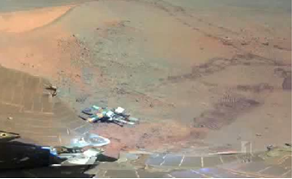
\includegraphics[width=35mm,height=35mm]{shota.png}  
		\label{fig:shota}	
	}
	\subfigure[]{
		\centering
		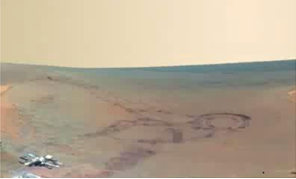
\includegraphics[width=35mm,height=35mm]{shotb.png}  
		\label{fig:shotb}
	}	
	\subfigure[]{
		\centering
		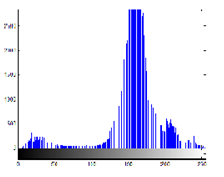
\includegraphics[width=35mm,height=35mm]{shotc.png}  
		\label{fig:shotc}	
	}
	\subfigure[]{
		\centering
		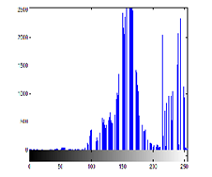
\includegraphics[width=35mm,height=35mm]{shotd.png}  
		\label{fig:shotd}
	}
	\caption{Example of a scene transition which is a soft cut that is undetected by color histogram method. a) and b) are two contiguous frames and b) is a scene transition boundary. c) and d) are the red channel histograms of a) and b) respectively. } \label{fig:shot}	
\end{figure}




